% Definicja klasy dokumentu
\documentclass[10pt, a4paper]{report}

% Pakiety
\usepackage{amsfonts}
\usepackage{amsmath}
\usepackage{amssymb}
\usepackage{caption}
\usepackage{fancyhdr}
\usepackage{geometry}
\usepackage{graphicx}
\usepackage[hidelinks]{hyperref}
\usepackage{indentfirst}
\usepackage[utf8x]{inputenc}
\usepackage{multirow}
\usepackage[MeX]{polski}
\usepackage{ucs}

\renewcommand{\maketitle}{
	\begin{titlepage}
		
		\begin{center}
			\vspace*{1cm}
			\noindent \rule{\linewidth}{0.4mm}
			\LARGE \textsc{Sterowanie pojazdem kołowym za pomocą gestów ręki}
			\rule{\linewidth}{0.4mm}
			\vspace*{3cm}
			
			\Large
			\textsc{Sterowniki robotów}
			
			\large
			\vspace*{2cm}
			\textsc{Patrycjusz Auguścik, 226523}\\
			\textsc{Maciej Kajdak, 226256}\\
			
			\vspace*{2cm}
			\textsc{prowadzący}\\
			\textsc{Mgr inż. Wojciech Domski}\\
			\vspace*{1.5cm}
			\textsc{\today}
			
		\end{center}
		
	\end{titlepage}
	\newpage}


\renewcommand*\thesection{\arabic{section}}


\newgeometry{tmargin=2cm, bmargin=2cm, lmargin=2cm, rmargin=2cm}

\begin{document}
	\maketitle
	\tableofcontents
	
	
	\newpage
	\section{Opis projektu i założenia projektowe}
\subsection{Projekt nadajnika wykorzystującego akcelerometr do sterowania pojazdem kołowym}
Projekt zakłada wykorzystanie akcelerometra dostępnego na płytce rozwojowej STM32L476 Discovery do sterowania pojazdem kołowym. Jest to moduł MEMS LSM303CTR z wbudowanym akcelerometrem i magnetometrem. Mikrokontroler będzie łączył się z modułem za pomocą szeregowego  interfejsu urządzeń peryferyjnych -- SPI w trybie Master Receives Only. Komunikacja między samochodzikiem a płytką odbywać się będzie za pomocą układu WiFi + Bluetooth BLE ESP-WROOM-32 - SMD. Z modułem mikrokontroler będzie się łączył dzięki komunikacji UART. W naszym projekcie zostanie wykorzystany tylko moduł bluetooth. Moduł ten w tej części projektu będzie pełnił rolę nadajnika. Pojazd będzie się poruszał w kierunku wskazanym przez dłoń sterującego. Aby połączyć się z samochodzikiem, należy trzymać w dłoni płytkę uruchomieniową, która będzie się łączyć z samochodzikiem automatycznie. 
Możliwości ruchu pojazdu:
\\* -- do przodu
\\* -- do tyłu
\\* -- w lewo
\\* -- w prawo
\\* Prędkość samochodzika będzie uzależniona od szybkości ruchów ręki.


\subsection{Projekt odbiornika i pojazdu kołowego}
Projekt zakłada wykorzystanie układu WiFi + Bluetooth BLE ESP-WROOM-32 - SMD. Z tego modułu zostanie wykorzystany tylko moduł bluetooth jako odbiornik informacji z nadajnika. Do zbudowania pojazdu zostanie wykorzystany stary samochodzik - zabawka. W celu ulepszenia samochodu - zamontujemy nowe silniczki komutatorowe prądu stałego. Pojazd ten będzie mógł osiągnąć dużą prędkość dzięki przekładni 2:1. Wmontujemy również czujniki odległości, a zadaniem pojazdu będzie natychmiastowe zatrzymanie się w przypadku napotkania przeszkody lub w momencie utraty połączenia bluetooth z nadajnikiem.
W opisywanym samochodziku wykorzystamy napęd na przednią oś, silniki zostaną połączone z mostkami H, a całością będzie sterować mikrokontroler.

\section{Harmonogram pracy}
\begin{table}[!h]
	\centering
	\begin{tabular}{|r|l|} \hline
		\textbf{Termin} & \textbf{Zadanie} \\ \hline \hline
		13.03 & wybór tematu projektu \\ \hline
		10.04 & opis projektu \\ \hline
		24.04 & \textbf{KM} schematy elektroniczne oraz model 3D pojazdu \\ \hline
		8.05 & rozwój modułu komunikacji z czujnikami odległości oraz silnikami \\ \hline
		22.05 & \textbf{KM} wstępne testy poprawności działania \\ \hline
		29.05 & poprawa ewentualnych błędów \\ \hline
		12.06 & \textbf{KM} w pełni działający robot. Poprawna komunikacja bluetooth \\
		& oraz reakcja pojazdu na przeszkody \\ \hline
	\end{tabular}
	\caption{Harmonogram zadań; KM -- kamień milowy}
\end{table}

\newpage
	\section{Schematy elektroniczne}
	\begin{figure}[!h]
		\centering
		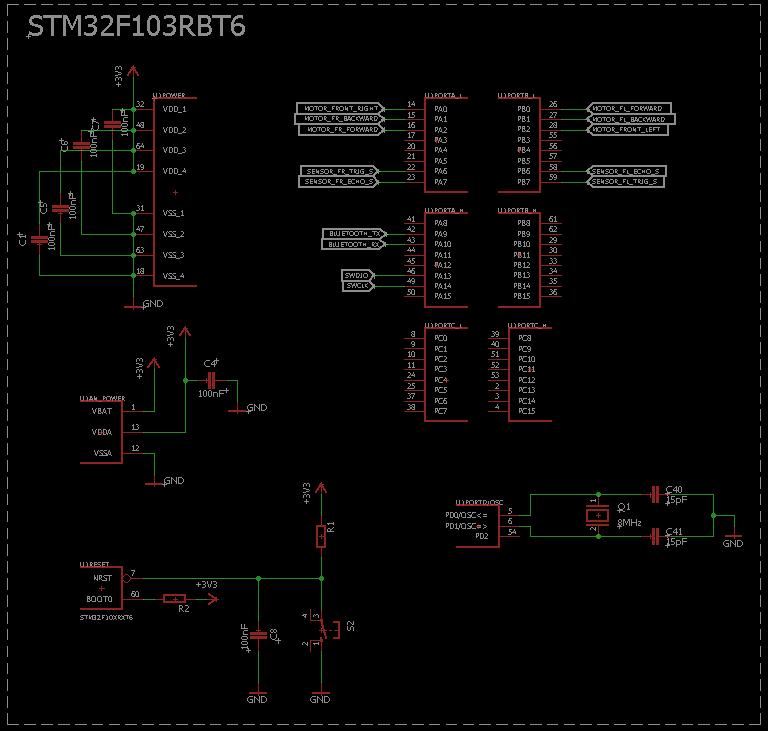
\includegraphics[scale=0.5, width=\textwidth ,height=\textheight ,keepaspectratio]{STM32.png}
		\caption{Schemat połączeń STM32F103RBT6}
	\end{figure}

\begin{figure}[!h]
	\centering
	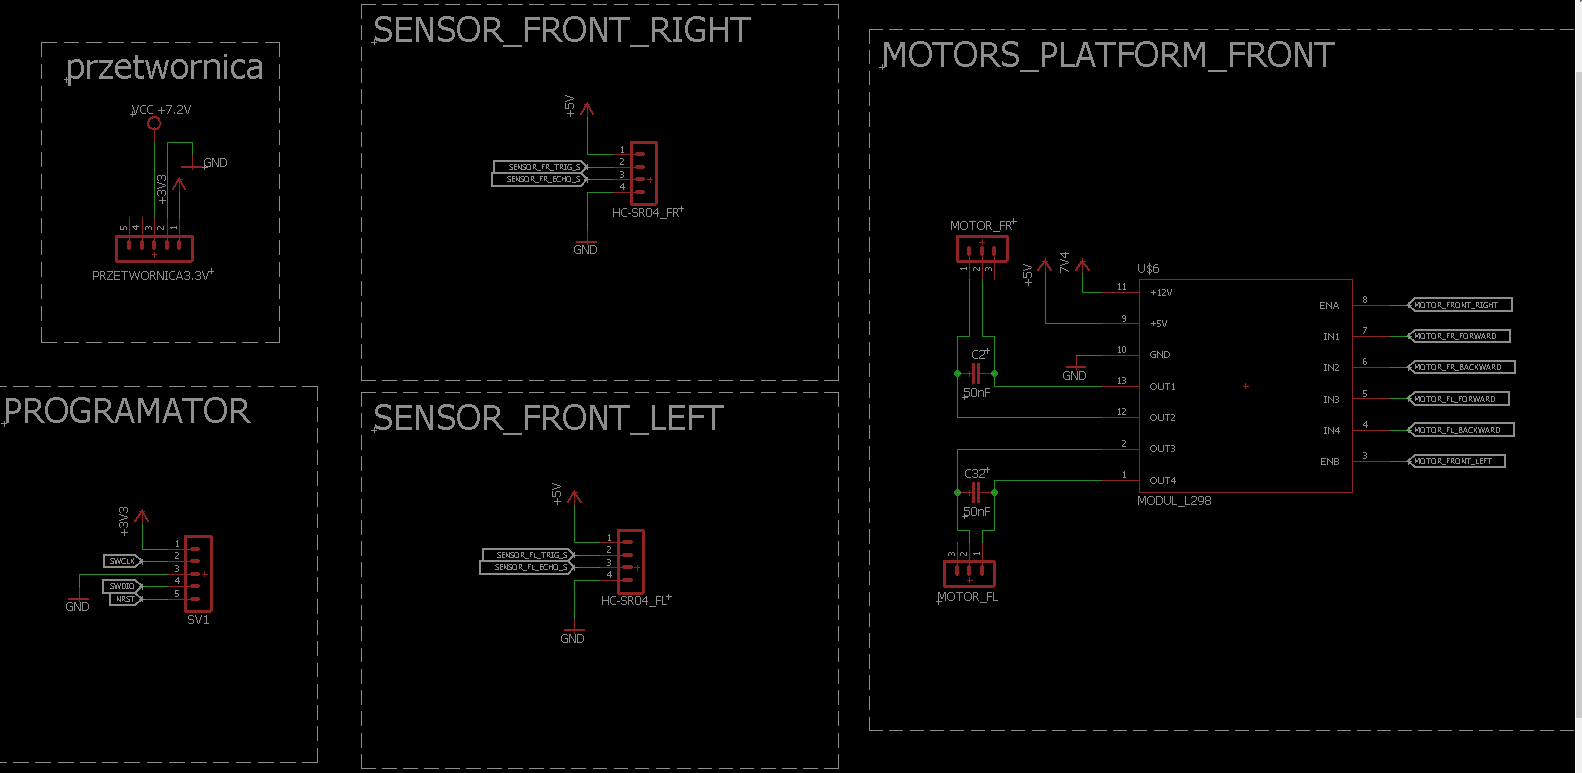
\includegraphics[scale=0.5, width=\textwidth ,height=\textheight ,keepaspectratio]{czujniki.png}
	\caption{Schemat połączeń programatora, czujników odległości oraz mostka H}
\end{figure}



\end{document}